%; whizzy chapter
% -initex iniptex -latex platex -format platex -bibtex jbibtex -fmt fmt
% 以上 whizzytex を使用する場合の設定。


%     Tokyo Debian Meeting resources
%     Copyright (C) 2006 Junichi Uekawa

%     This program is free software; you can redistribute it and/or modify
%     it under the terms of the GNU General Public License as published by
%     the Free Software Foundation; either version 2 of the License, or
%     (at your option) any later version.

%     This program is distributed in the hope that it will be useful,
%     but WITHOUT ANY WARRANTY; without even the implied warranty of
%     MERCHANTABILITY or FITNESS FOR A PARTICULAR PURPOSE.  See the
%     GNU General Public License for more details.

%     You should have received a copy of the GNU General Public License
%     along with this program; if not, write to the Free Software
%     Foundation, Inc., 51 Franklin St, Fifth Floor, Boston, MA  02110-1301 USA

%   Pdf作成手順
% dvipdfmx debianmeetingresume200606.dvi
%  preview (shell-command (concat "xpdf " (replace-regexp-in-string "tex$" "pdf"(buffer-file-name)) "&"))
% 画像ファイルを処理するためにはebbを利用してboundingboxを作成。
%(shell-command "cd image200612; ebb *.png")

%%ここからヘッダ開始。

\documentclass[mingoth,a4paper]{jsarticle}
\usepackage[dvipdfmx]{graphicx}
\usepackage{fancybox}
\usepackage{longtable}
\usepackage{ascmac}	% 囲み (screen,itembox)
\usepackage{fancyvrb}   % 囲み Verbatim のために必要
\usepackage[dvipdfmx]{hyperref}
\usepackage{url}
\usepackage[dvipdfmx]{color}

%http://www.naney.org/diki/dk/hyperref.html
%日本語EUC系環境の時
\AtBeginDvi{\special{pdf:tounicode EUC-UCS2}}
%シフトJIS系環境の時
%\AtBeginDvi{\special{pdf:tounicode 90ms-RKSJ-UCS2}}

%% spacing の設定をする。外枠を減らす。
\setlength\headheight{0mm}
\setlength\topmargin{-20mm}
\setlength\headsep{0mm}
\setlength\topskip{3mm}
\setlength\maxdepth{4pt}
\setlength\columnsep{6mm}
\setlength\textheight{252mm}
\setlength\topmargin{-5mm}
\setlength\textwidth{170mm}
\setlength\oddsidemargin{-5mm}
\setlength\evensidemargin{-5mm}

% commandline環境を定義。画面入出力についてはcommandline環境
% で表記する
\newenvironment{commandline}%
{\VerbatimEnvironment
  \begin{Sbox}\begin{minipage}{15cm}\begin{fontsize}{7.3}{7.3} \begin{BVerbatim}}%
{\end{BVerbatim}\end{fontsize}\end{minipage}\end{Sbox}
  \setlength{\fboxsep}{8pt}\fbox{\TheSbox}}


%%% start of santaku
\makeatletter
\newwrite\tf@jqz
\immediate\openout\tf@jqz\jobname.jqz\relax
\makeatother
\newcounter{santakucounter}
\newcommand{\santaku}[5]{%
\addtocounter{santakucounter}{1}

\addtocontents{jqz}{\arabic{santakucounter}. #5\\}
\begin{minipage}{1\hsize}
問題\arabic{santakucounter}. 
#1\\
□ A #2\\
□ B #3\\
□ C #4
\end{minipage}
\hspace{1cm}
\\

}
%%% end of santaku

\newcommand{\emptyspace}{(\underline{\hspace{1cm}})}

\newcommand{\subsubsubsection}[1]{%
\vspace{1zw}{\bf #1}\\}


% sectionをセンタリングする
\makeatletter
  \renewcommand{\section}{\@startsection{section}{1}{\z@}%
    {\Cvs \@plus.5\Cdp \@minus.2\Cdp}% 前アキ
    {.5\Cvs \@plus.3\Cdp}% 後アキ
    {\normalfont\Huge\headfont\raggedright\centering}} % style
\makeatother

% section の代わりの環境
\newcommand{\dancersection}[2]{%
\newpage
東京エリアDebian勉強会 2006
\hrule
\vspace{0.5mm}
\hrule
%\hfill{}
\includegraphics[width=3cm]{image200502/openlogo-nd.eps}\\
\hfill{}
\includegraphics[width=16cm]{image2006-natsu/guruguru-sand-light.png}\\
\vspace{-5cm}
\begin{center}
\section{#1}
\end{center}
\hfill{}\colorbox{white}{#2}\hspace{3cm}\space\\
\vspace{1cm}
\hrule
\vspace{0.5mm}
\hrule
\vspace{1cm}
}

% for dancerj
\newcommand{\fgref}[1]{図\ref{#1}}
\newcommand{\tbref}[1]{表\ref{#1}}


\begin{document}

\begin{titlepage}

% 毎月変更する部分, 本文の末尾も修正することをわすれずに
\title{
 第23回 東京エリア Debian 勉強会\\事前資料}
\date{2006年12月16日}
\author{Debian勉強会会場係 上川 純一\thanks{Debian Project Official Developer}} 
\maketitle
\thispagestyle{empty}
\end{titlepage}

\newpage
\tableofcontents

\dancersection{Introduction To Debian 勉強会}{上川 純一}

今月のDebian勉強会へようこそ。
これからDebianのあやしい世界に入るという方も、すでにどっぷりとつかってい
るという方も、月に一回Debianについて語りませんか?

目的として下記の二つを考えています。

\begin{itemize}
 \item メールではよみとれない、もしくはよみとってられないような情報を情
       報共有する場をつくる
 \item まとまっていないDebianを利用する際の情報をまとめて、ある程度の塊と
       して出してみる
\end{itemize}

また、東京にはLinuxの勉強会はたくさんありますので、Debianに限定した勉強
会にします。Linuxの基本的な利用方法などが知りたい方は、他でがんばってくださ
い。
Debianの勉強会ということで究極的には参加者全員がDebian Packageを
がりがりと作りながらスーパーハッカーになれるような姿を妄想しています。

Debianをこれからどうするという能動的な展開への土台としての空間を提供し、
情報の共有をしたい、というのが目的です。
次回は違うこと言ってるかもしれませんが、御容赦を。

\subsection{講師紹介}

\begin{itemize}
 \item{上川 純一} 宴会の幹事です。
\end{itemize}

\subsection{事前課題紹介}

今回の事前課題は
「来年のDebian勉強会でやりたいこと」もしくは「来年の
Debian勉強会のスタイルを提案する」
というタイトルで200-800文字程度の文章を書いてください。というものでした。
その課題に対して下記の内容を提出いただきました。

\subsubsection{小林儀匡さん}

『来年のDebian勉強会のスタイルを提案する』

Debian勉強会もついに2歳を迎え、パッケージ作成作業に関連する各種ツールの
使い方・Debian Policy Manualの内容・翻訳作業などといった、開発者への入口
となる情報を提供するテーマは一通り扱ったと思います。それらの内容に大きな
変化があったらそれは更新する必要がありますし、まだ触れられていないツール
についても扱う必要があると思いますが、開発者への入口をまとめたドキュメン
トの提供という当初の大きな目的の一つ\footnote{というのは自分の勝手な思い
込みかもしれませんが。}は大方達成されたのではないでしょうか。

このような状況を鑑みると、これからは、「現在のDebian GNU/Linuxシステムに
存在する問題点を何かしら見つけて、それについてグループディスカッションの
ようなかたちで掘り下げ、今後の開発作業に繋げてみる」という問題発見型の勉
強会も必要になるのではないかと思います。これまでも飲み会で「あれはどうに
かならないか」と議論になったり、ネットワークの設定についての課題への回答
を巡って議論になったりしましたが、このような議論をきちんとしたかたちでやっ
てみる、ということです。理想的には (かなり大きな理想ですが)、本勉強会で
議論したことをDebian本家のメーリングリストに英語で流して、それを元に何か
を生み出せればとても素敵だと思います。もちろん、これを毎月行うのはやや負
担が大きく、実際の作業がなかなか進まないままネタ切れというのがオチになる
可能性もあるので、これまでのように、会議の報告や「Debianでこんなことをし
てみた」というネタ的な話、開発関連ツールではないがまとめておくと有用な事
項 (glibc・Flash・マルチメディア関連・……) のまとめなども混ぜていく必要
があるかと思いますが……。

ネタがなくなって勉強会自体がマンネリ化しだらだら続くことのないよう、自分
ももう少し提供できるネタがないか考え、そして実際に提供しながら臨みたいと
思う2006年冬です。

\subsubsection{前田 耕平さん}


お題「来年のDebian勉強会のスタイルを提案する」として、ワークショップ形式
で議論するのが良いですね。他の参加者の方と(宴会以外で)話す機会も増えま
すので。って、今回はもろにそういう形式のようですね。失礼しました。

あとは、ハンズオンとか。帰宅後に資料を見てやるのも良いのですが、宴会の後、
帰宅したら寝てしまうので、やはりその場で手を動かす方がより効果が高いかと。
(次の日だと忘れるか、覚えていてもやらない、という事もままあるので…)

\subsubsection{澤田さん}

スタイルの提案で書きます。「/etc/network/interfacesをさらしてください」
という事前課題はいろいろバッドノウハウが出て盛り上がったことと思われます
(諸事情により参加しませんでしたが)。

そこで今後も、ある事項について、「私はこうやっています」という事前課題を
書いてもらい、バッドノウハウとしてまとめるというのはどうでしょうか?例え
ば、「apt-get upgradeしたらパッケージが壊れていてアップグレードが完了し
ない。怒りのBTSは当然投げるとして、とりあえずどう対処する?」とか、「バッ
クアップ、何使ってますか?何バックアップしてますか?」(「バックアップ 
Debian」でググるとやまねさんの過去の投稿がありますね)とか、知っている人
は知っているというバッドノウハウが多いと思います。


\subsubsection{小室 文さん}

「来年のDebian勉強会でやりたいこと」
勉強会でやりたい事ではないですが、女の子の参加者がもっと増えるように地道
な活動?をしようと決めてます。いないはずはないので、勉強会に来てもらえる
ようにいろんな所で探したいと思います。


「来年のDebian勉強会のスタイルを提案する」
継続して多くの人が参加しないのは、参加者のレベルに(しょうがない事ですが)
バラツキがある為だと思います。ちょっと分からない単語や内容を後で調べてみ
よう、というレベルの開きではなくて、何の事かすら分からない事が時々ありま
す(特にカーネル関係は難しい…)。debian勉強会+初級・中級者向け勉強会が
あったら、利用者も増えて階段を上る感じでいいかもしれません。
(有志なので難しいとは思いますが。。。)

\subsubsection{キタハラさん}

    現在のDebian勉強会のスタイルに不満点は無いので
すが・・・

    最近、初心者向けの某勉強会で輪読していて、20
ン年前の学生時代の雰囲気を堪能して来ました。

    輪読は、対象となる資料を「事前に読んで」おき、
その時に理解できなかった所や疑問に思った所を、当日
「有識者と共に」ディスカッションする事により、「他
の参加者の視点」と共に対象の事柄を「より深く理解」
できるという利点があると思います。

    現在のDebian勉強会で輪読を行うのは、少々無理が
あるかもしれませんが(別枠で初心者向け『徹底入門
第4版 〜etch対応(仮?)』の輪読(読書会)があった
ら参加したいなぁ〜)、適当な長さの資料を事前に読ん
でおき、当日参加者が順番に読んで、疑問点や注意点を
話し合うコーナーを作るという形ならば、実現可能かも
しれません。

\subsubsection{青木さん}

「来年のDebian勉強会でやりたいこと」というお題をいただきましたので
おひとつ話させていただきます。

今までDebian勉強会に関して開催形態(課題があること)に減らず口を叩いた
以外出席すらしてきていない私がDebian勉強会で何をするかを語るのもチョッと
変な気がします。

でもソフト関係で食ってるわけでもないわたしが今までDEBIANでいろいろしてきた
経験を、長く終わりの見えないNMプロセスに取り組もうとされている方々と共有す
る機会がもてればいいのではないかと考えています。

それにDEBIANは英語でのコミュニケーションがDDとして続く必須条件という状況
もあります。これって多くの日本人にとって結構気の重いものでは無いでしょうか?

これらの障害のあるDEBIANですが、だからこそ日本人が参加し、日本語環境を世界
中どこにいても誰でも使えるようにしようではありませんか?いま日本語環境をサ
ポートしているひとは少ないので、是非協力してくれるひとを見付けたいものです。

それから、内容が古くなったのが否めないDEBIAN REFERENCEをもう少しバージョン
アップに影響されないようにしたかたちにする、そしてXMLに変更する作業をどな
たか見付けられないかなという勝手な期待もあります。

\subsubsection{上川}

勉強会のスタイルは、理由があってこうなっている部分もありますが、最初にこ
うしたからこうなっている、ということで特に理由があって決まっていない部分
もあります。たまにはそういう部分に変化を加えていかないと、マンネリになっ
てしまい、飽きてくるので、変化させることは重要だと思っています。是非みな
さまのアイデアを活用して何か違う形を採り入れたいとおもっております。


%%% trivia quiz
\dancersection{Debian Weekly News trivia quiz}{上川 純一}

ところで、Debian Weekly News (DWN)は読んでいますか?
Debian 界隈でおきていることについて書いているDebian Weekly News.
毎回読んでいるといろいろと分かって来ますが、一人で読んでいても、解説が少
ないので、
意味がわからないところもあるかも知れません。みんなでDWNを読んでみましょう。

漫然と読むだけではおもしろくないので、DWNの記事から出題した以下の質問にこたえてみてください。
後で内容は解説します。

\subsection{2006年41号}
\url{http://www.debian.org/News/weekly/2006/41/}
にある11月28日版です。

\santaku
{Debian Conference 7 日程が決まりました。いつからでしょうか。}
{4/1}
{5/22}
{6/17}
{C}


\santaku
{Debian Project に新しい開発用マシンが導入されました。どのマシンでしょうか。}
{Sun Fire T2000}
{Sony Playstation 3}
{TiVo Series2 DVR}
{A}


\dancersection{最近のDebian関連のミーティング報告}{上川 純一}

\subsection{東京エリアDebian勉強会22回目報告}
% (query-replace-regexp "<.*>" "")

2006年11月19日に第22回Debian勉強会を実施しました。Sid の使いかたについて、
	    Debian BTS の紹介、パッケージの作り方についての紹介を行いま
	    した。今回は関西開催です。今回の参加人数は20人くらいでした。
	    参加者は出欠をとっていないので正確にはわかりませんが、藤澤さ
	    ん、畑中さん、浜辺さん、乾さん、亀谷さん、谷口さん、久松さん、
	    岩松さん、山下さん、榎さん、岩本さん、さとうまことさん、小森
	    さん、やまねさん、上川でした。
	  
	    まず、事前課題の紹介をしました。
	    Debian についての疑問や、今後の Debian Project への気概が感じられました。
	    今回は、事前課題の紹介が盛り上がりすぎて、クイズをするのを忘れていました、ごめんなさい。
	  
	    上川が sid の使いかたについて紹介しました。
	    apt-listchangesはデフォルトでは root にメールを送ってくれるという仕組になっていますが、
	    dpkg-reconfigure apt-listchanges で設定してあげると、
	    インストール前に changelog を提示してインストールするかどうかを質問してくれるので、
	    是非みなさんそういうつかいかたをしましょう、という話が出ました。
	  
	  
	    上川が Debian BTS の使いかたについて紹介しました。仕組とか
	    裏側のマニアックな話の概要だけを紹介しただけでしたので、今
	    後さらに深みにはまっていく必要があります。
	  
	  
	    岩松さんが、パッケージの作り方を cairo-dock パッケージを例に
	    して紹介していました。わかりやすい説明にみんなパッケージをが
	    んがん作れるようになったようです。
	  
	    今回宴会は「One's」で行いました。勉強会の会場から京橋の宴
	    会会場まで40分くらいかかりましたが、無事遭難せずに到達でき
	    ました。結婚式の二次会を裏でやっていた司会の声がうるさかっ
	    たので、今後は結婚式の二次会をやらないような店を選んだ方が
	    よいかもしれませんね。
	  
  
	    今回の企画は大阪電気通信大学の久松先生の全面的な御協力をい
	    ただき実現しました。ありがとうございました。
	  

\subsection{関西オープンソース Debian BOF}
% (query-replace-regexp "<.*>" "")

2006年11月18日・19日関西の関西オープンソースの中でDebian BOFを11月19日午
後に開催しました。岩松さん、山根さん、上川で発表しました。Debian Project 
の紹介、 Debian JP の紹介、そして、Debian etch がどういうものになるのか、
という紹介をしました。会場では Debian ユーザが30人程度参加しました。個人
的には、knoppix ベースのマルチメディア向けディストリビューションを開発し
ているのがじゅんさんにお会いできたのが印象的でした。

\dancersection{Debian勉強会資料の作成方法}{上川 純一}
\label{sec:debmtg2006res}

\subsection{レポジトリを取得し、パッケージの準備を行う}

レポジトリをチェックアウトします。

\begin{commandline}
$ cvs -d :ext:cvs.alioth.debian.org:/cvsroot/tokyodebian . 
\end{commandline}

ディレクトリ構成は次のようになっています。

\begin{itemize}
 \item monthly-report: TeXのソースが全部フラットにおいてあります。ファイ
       ル名は、 debianmeetingresumeYYYYMM.texという名前になっています。
       プレゼンテーションファイルは
       debianmeetingresumeYYYYMM-presentation.tex という名前になってい
       ます。
       \begin{itemize}
	\item imageYYYYMM:各月用の画像ファイル
	\item debian: デビアンパッケージ用ディレクトリ
       \end{itemize}
 \item muse: ウェブ(wiki)
 \item meetinglog: 議事録置場
\end{itemize}

ビルドに必要なパッケージをインストールします。

\begin{commandline}
apt-get install ptex-bin dvipdfmx latex-beamer \
 okumura-clsfiles gs-esp xpdf xpdf-japanese 

\end{commandline}

編集に便利なツールもついでにインストールしてみてもよいでしょう。

\begin{commandline}
 apt-get install whizzytex advi emacs21 yatex
\end{commandline}

\subsection{pLaTeXで文書作成}

make コマンド一発で 
PDFファイルまで、コンパイルすることができます。
Makefile には、あらゆる debianmeeting*.texファイルに関して .pdf ファイルを作成するよう
にルールが作成されています。

注意する点として、印刷を考え、ページ数が4の倍数になるようにしてください。

\begin{commandline}
SOURCE:=$(wildcard debianmeeting*.tex)
DVIFILES:=$(SOURCE:%.tex=%.dvi)
PDFFILES:=$(SOURCE:%.tex=%.pdf)
all: $(PDFFILES)

%.pdf: %.dvi
	dvipdfmx $< 

%.dvi: %.tex
	# check kanji-code of the tex file.
	iconv -f iso-2022-jp -t iso-2022-jp < $< > /dev/null
	platex $<
	platex $<
	platex $<

clean:
	-rm *.dvi *.aux *.toc *~ *.log *.waux *.out _whizzy_* *.snm *.nav *.jqz

\end{commandline}


\subsubsection{画像ファイルの処理}

画面写真の画像を追加するときは、できるだけサイズの小さい png などを利用
してください。グラフなどの線画であれば、epsでかまいません。png であれば、 
ebb コマンドを利用してbounding box を作成してください。

\begin{commandline}
 ebb XXX.png
\end{commandline}

ps であれば、 eps2epsでバウンディングボックスを追加してあげるとうまくい
きます。sodipodi の出力する ps を eps2epsで処理すれば sodipodi で画像を
作成することができます。

\subsection{pLaTeX+latex-beamerで文書作成}

残念ながら whizzytex でプリビューはうまく動かないです。

がりがりと作成し、xpdfでプリビューしながらがんばって作成してください。


\subsection*{参考:Debian 勉強会のウェブインタフェース}

Debian 勉強会のウェブインタフェースについて解説します。

初期は
\url{http://www.netfort.gr.jp/~dancer/column/2005-debianmeeting.html.ja} 
にあるページを手動で生成していました。

CMSを採用したいところでしたが、CMSを探索している間中ずっと手動で生成して
いるのも困難なので現状のページにかわりました。
\url{http://tokyodebian.alioth.debian.org/2006-11.html} のようなページに
なっています。

該当するファイルはCVSレポジトリの muse/ ディレクトリにあります。emacs を 
wiki 処理系として利用しており、 Makefile から emacs を呼出し、HTML を静
的に生成するようになっています。

今後実現していきたい内容としては
\begin{itemize}
 \item RSSをはくアナウンスページ
 \item ユーザ参加登録と同時に事前課題登録
 \item 事後のアンケート
 \item 登録ユーザへの次回通知
 \item 事後の資料公開・感想文公開
\end{itemize}

があります。

muse-el は一般的な構成ではなく開発もあまり活発でないので、今後利用ツール
を変更したいと考えています。

\dancersection{Debian勉強会2006年結果統計}{上川}
\label{sec:debmtg2006}

\subsection{Debian勉強会評価項目}

Debian の開発者を増やしていき、Debian の活動を活発にしていきたい、そうい
う思いでDebian 勉強会は開催しています。
そもそも Debianのユーザの裾野がひろがり、活発なユーザが増え、
ユーザが開発者になろう、と思って、NMプロセスを通らないと、Debian Developer は増
えません。

%sodipodi経由、eps2epsで作成
% eps2eps hierarchy.ps hierarchy.eps
\includegraphics[width=0.5\hsize]{image200612/hierarchy.eps}

Debian 勉強会が成功した、という場合、何がおきた場合でしょうか。

\begin{itemize}
 \item 直接貢献: バグがどんどんクローズされていき、新機能が追加
 \item 各種アプリケーションの日本語対応が進捗
 \item 日本から Debian Developer を生み出す
 \item 日本の Debian ユーザが増える
 \item すでに経験の豊富な Debian Developer の知識を展開
 \item ドキュメントが増える
\end{itemize}

直接評価できる指標としては下記があるでしょう。

\begin{itemize}
 \item 日本語で増えたドキュメント数
 \item Debian Developer の参加者数
 \item Debian Developer でない参加者数
 \item 新規の参加者
 \item 新規に参加して二度以上参加してくれた参加者の数
\end{itemize}

それでは、値がどういうものか見てみましょう。

概算の値なので、正確ではありません。過去の記録を発掘して、今後の検討のた
めにひねり出しているものです。

\subsection{新規の参加者}

\begin{itemize}
 \item 2005年1月: 20 人
 \item 2005年2月: 6 人
 \item 2005年のこり: 12 人
 \item 2006年 -6月: 9人
 \item 2006年 -10月: 14人
\end{itemize}

\subsection{新規に参加して二度以上参加してくれた参加者の数}

参加者の統計です。

\begin{itemize}
 \item 2005年: 39人中 21人
 \item 2006年上半期 (-6月): 9人中 5人
 \item 2006年下半期 (-10月): 14人中 2人
\end{itemize}

\subsection{Debian Developer比率}

のべ参加者の中からのおおよその分析ですが、どれくらいの参加者が Debian
Developer で、どれくらいの参加者が New Maintainer Queue に入っているか、
の統計です。

\begin{itemize}
 \item 2005年:39人中 DD 4 人? NM 3 人
 \item 2006年 -10月:36人中 DD 6 人 NM 6 人
\end{itemize}

\subsection{参加人数}

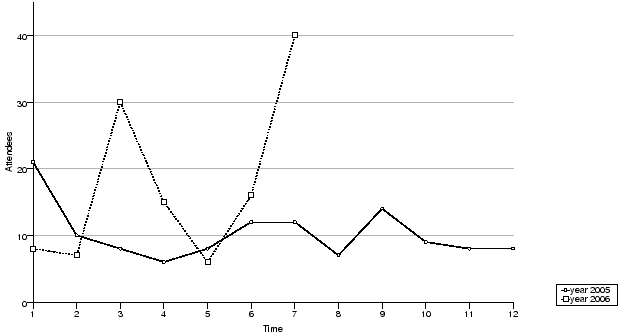
\includegraphics[width=1\hsize]{image200612/people-chart.png}

 
 \begin{table}[ht]
\begin{minipage}{0.6\hsize}
 \caption{参加人数(2006年)}\label{tab:count2006}
 \begin{center}
  \begin{tabular}{|l|c|l|}
 \hline
 & 参加人数 & \\
 \hline
 2006年1月 & 8 & policy,Debian勉強会でやりたいこと\\
 2006年2月 & 7 & policy, multimedia \\
 2006年3月 & 30 & OSC: debian勉強会,sid \\
 2006年4月 & 15 & policy, latex \\
 2006年5月 & 6 & mexico \\
 2006年6月 & 16 & debconf, cowdancer\\
 2006年7月 & 40 & OSC-Do: MacBook Debian \\
 2006年8月 & 17 & 13執念 \\
 2006年9月 & 12 & 翻訳、Debian-specific、oprofile \\
 2006年10月 & 23 & network, i18n会議、Flash、apt \\
 2006年11月 & 20 & 関西: bug, sid, packaging \\
 2006年12月 & 14 & 忘年会 \\
 \hline
  \end{tabular}
 \end{center}
\end{minipage}
\begin{minipage}{0.35\hsize}
 \caption{参加人数(2005年、概算)}\label{tab:count}
 \begin{center}
  \begin{tabular}{|l|c|}
   & 参加人数 \\
 \hline
   2005年1月 & 21 \\
   2005年2月 & 10 \\
   2005年3月 (早朝)& 8\\
   2005年4月 & 6\\
   2005年5月 & 8\\
   2005年6月 & 12\\
   2005年7月 & 12\\
   2005年8月 & 7\\
   2005年9月 & 14\\
   2005年10月 & 9\\
   2005年11月 & 8\\
   2005年12月 & 8 \\
  \end{tabular}
 \end{center}
\end{minipage}
 \end{table}

\subsection{実施テーマ}

今年は下記のテーマを実施しました。
\begin{itemize}
 \item Debian weekly news クイズを隔月で
 \item グループワーク:Debian勉強会でやりたいこと
 \item Debian Policy 入門
 \item Debian Multimedia Project
 \item Debian 勉強会紹介
 \item sid のすすめ
 \item LaTeX 
 \item DebConf2006 報告
 \item cowdancer 
 \item MacBook Debian
 \item module-assistant
 \item oprofile
 \item 翻訳のすすめ
 \item Debian-specific
 \item i18n
 \item Flash
 \item Bug tracking system
 \item Debian packaging.
\end{itemize}

\subsection{会議の構成}

今年のDebian 勉強会にはおおきくわけて三種類の会議形態がありました。

\begin{itemize}
 \item OSC(春、秋)
 \item 出張(OSC北海道、メキシコ、KOF)
 \item 通常
\end{itemize}

東京のOSCでの開催は、通常の勉強会に参加するよりハードルを低く設定してい
ます。できるだけ多くの人たちに参加してもらうことを目的としています。これ
でDebian勉強会の雰囲気をしってもらい、興味を持ってもらい、通常の勉強会に
参加しやすくなるように配慮しています。

Debian 勉強会は、ふたつの目的をもっています。そのふたつの目的にあわせた
会議設定をしています。一つめはDebian 開発者の開拓です。二つ目はDebianユー
ザの集まる場所を提供することです。

OSC, KOF など、年三回程度のイベントにおいては、他の主催者の企画したイベ
ントのうえでイベントを実施しています。コストも、集客方法も主催者側に一任
しています。また、実務上、事前課題の設定などもできていません。

毎月実施している勉強会については、より目的意識の高い会として位置づけてい
ます。Debian 開発の側に参画し、よりドキュメントを生成する側にまわり、み
んなでDebianの現在の課題についてブレーンストーミングできるようになること
が目標です。そのため、事前課題を準備して、目的を共有できるような仕組を準
備しています。

また、現状の勉強会の運営については、毎年一回、12月開催の勉強会に確認し、
来年度の運営方針を確認することにしています。


\dancersection{Debian勉強会2006年、作業フロー}{上川}
\label{sec:debmtg2006flow}

どういう作業をしたでしょうか。書き出してみましょう。

\subsection{年に一回の作業}

\begin{itemize}
 \item 年次計画を仮決め、毎月どの日に開催するのかを決定して、
       それをベースにしてその後の議論をする。
 \item tokyodebian-2006 メーリングリストの作成
\end{itemize}

\subsection{事前準備}

\begin{itemize}
 \item 開催二ヵ月前: 開催場所の予約
 \item 資料の作成
 \item 開催二週間前: \url{http://utage.org/enkai} 宴会君への登録
 \item 開催二週間前: \url{http://tokyodebian.alioth.debian.org/} ウェブサイトの更新
 \item 開催二週間前: mixi と debian-users/debian-devel にアナウンス
 \item 開催二日前:印刷、資料は4の倍数のページ数にして、kinko's にコピー
       依頼。\footnote{2006年10月、ウェブベースで依頼してみたところ無事印刷された
       ので、今後はウェブで依頼する予定。}
 \item 開催一日前:宴会場所の予約
\end{itemize}

\subsection{事後処理}

\begin{itemize}
 \item 議事録の作成
 \item blogトラックバックの収集
\end{itemize}

\newpage
\dancersection{Bug Squashing Party}{岩松 信洋}
\subsection{はじめに}
今回 Debian JP Project で Bug Squashing Party を行いました。
その内容と報告をまとめました。
 
\subsection{Bug Squashing Party とは?}
Bug Squashing Party\footnote{http://wiki.debian.org/BSP} とはバグつぶし大会のことです。
Debian の場合だと、stable のリリース前や定期的に行われています。
目的としては Release Critical Bug を減らしたり問題のあるパッケージを集中的に直したりします。

\subsubsection{Bug Squashing Party の重要な点}

Bug Squashing Party は以下の点を決める事が重要です。
\begin{itemize}
	\item 日時

		Bug Squashing Party をやる日時と開催期間を決める必要があります。
	\item 場所

		Bug Squashing Party を行う場所を決める必要があります。
		IRC だけでなく、場所を借りて Face to Face で話合いながら
		行う必要もあるからです。 
	\item コーディネーターおよび指揮官
		
		Bug Squashing Party を円滑に進めるため、指揮官が必要です。
		バグの情報を把握し、参加者に指示を行います。
		Debian の場合だと、Debian Release Manager や Release チームと話を進める
		ことがあります。このような場合には Release チームに名前が知られている人に
		コーディネーターになってもらったほうが話が進めやすくなるかもしれません。
\end{itemize}

\subsubsection{コーディネイター、指揮官が行うこと}
コーディネイター、指揮官は、以下の事について知っている必要があります。
\begin{itemize}
	\item Bug Squashing Party の目的を把握する
		
		ただ単にバグを潰すだけではなく、今回はinput method に関してのバグを潰す、といった
		目的があると全体の流れをコントロールしやすいと思います。

	\item 他で行われている Bug Squashing Party の主催者やコーディネイターと話をする。

		他で Bug Squashing Party をやっている可能性があるので、話をして無駄な作業を減らすよう
		動く必要があります。

	\item バグ対策の指示

		参加者にバグの対策を指示します。
		
\end{itemize}

\subsubsection{参加者が事前に知っておくこと}

参加者はただ単にバグを潰すという作業をするだけではなく Bug Squashing Party はどのような
ものなのか理解しておく必要があります。

また、Debian の場合は NMU\footnote{Non Maintainer Upload} を行う可能性が高いので、NMU時の
パッケージバージョンの付け方やChangelog の書き方を知っておく必要があります。
もちろん Debian Policy なども事前に読んで勉強しておく必要があります。:-)


参加者の中で Debian Developer の方がおられる場合は、Debian Developer ではない人が修正した
パッケージのアップロードしたり、いろいろ助言等をしていただけると助かるかもしれません。

\subsection{今回行われた Bug Squashing Party }

\subsubsection{今回の目的}
今回、Debian JP Project で Bug Squashing Party を行いました。
今回の目的は以下のものがあります。

\begin{itemize}
	\item etch リリース前なので、RC バグを潰したい
	\item Bug Squashing Party ってどのようなものなのか、ためしにやってみる
	\item Debian JP Project はちゃんと活動しています、というアピール
\end{itemize}

%ようするに、いろいろ初めてなので実験的にやろうという流れで行いました。

\subsubsection{今回の Bug Squashing Party の流れ}

どのような流れ、内容でおこなったのか以下にまとめました。

\begin{enumerate}
\item 事の発端

 OSC 2006 の帰りにgotom さん、上川さん、えとーさん、小林さん、私でサイゼリアで食事していたところ、上川さんが
「Bug Squashing Party やりたいねぇ。」から始まったが、この時点でだれが話を進めることにするか決まらない。

\item Debian JP IRC ミーティングで議論

 Debian JP で行われたミーティングで、私が話を進めることになる。

\item debian-devel@debian.or.jp で提案

 Debian JP Project が提供している開発用メーリングリストで提案。\footnote{[debian-devel:16525] Bug Squashing Party について}
 この投稿によるスレッドで武藤さんから助言を頂く。

\item コーディネイターを決める

 Bug Squashing Party を進めるコーディネイターをして、gotomさんに依頼。
 快諾していだく。

\item 開催日時を決める
 
 ちょうど11/23 (木) が休みだったので、この日にする。朝弱い人のために10時から行うことにした。
 このあたりは IRC で決めた気がするが、ログがない。
 開催内容は以下のとおり。


\begin{commandline}

日時
        2006 年  11 月 23 日 (木) 10:00 - 15:00

会場
        IRC
	IRC サーバー	: osdn.debian.or.jp
	IRC チャンネル	: #debianjp-bsp
	漢字コード	: iso-2022-jp

コーディネイター
	後藤 正徳さん

\end{commandline}


\item 開催告知
 
 debian-users@debian.or.jp および debian-devel@debian.or.jp に開催告知を流した。
 しかし、反応なし。

\item 開催

 無事開催。しかし人の集まりが悪い。
 人が集まり始めると gotom さんがいろいろ指示をしてくれて、順調に Bug Squashing Party は進んだ。
 
 進めるにあたって、参考にしたサイトは以下のとおり。
 \begin{itemize}
  \item Debian RC バグ曲線 

	\url{http://bugs.debian.org/release-critical/}
  \item 現在の RC バグ情報 
	
	\url{http://bugs.debian.org/release-critical/debian/all.html}
  \item リリースチームが使っている RC バグ管理サイト 
	
\url{http://bts.turmzimmer.net/details.php}
 \end{itemize}
\item 終了

 15 時に終了。かなり不完全燃焼。
 NMU するまでが Bug Squashing Party です。

\end{enumerate}

\subsubsection{結果}
 今回行われた Bug Squashing Party の結果は以下の通りです。

\begin{itemize}
 \item 参加者
   \begin{itemize}
   \item gotom
   \item iwamatsu
   \item ay\_
   \item Henrich
   \item mino
   \item dancerj
   \item nori1
   \item kmuto
   \item omote\_bot
   \item sato\_at\_deb-newb
   \item tyuyu
   \end{itemize}

 \item 活動内容
   \begin{itemize}
   \item xxdiff 修正 \debianbug{399764}
   \item qemu は問題なし \debianbug{399382}は close しても問題ない
   \item murasaki \debianbug{378318} hppa only
   \item libflash-mozplugin \debianbug{399508} arm/ia64 only
   \item rarpd \debianbug{395739}
   \item cowdancer \debianbug{384132}
   \item zoph \debianbug{398637}
   \item リリースノート追従
   \item po-debconf 更新
   \item rsjog
   \item bookview最新版ビルドしていま作業中、arm fix失敗
   \end{itemize}
\end{itemize}

\subsubsection{感想}

 Bug Squashing Party が終わったあと、IRC で意見交換を行いました。

\begin{itemize}

    \item 5時間は短い。重いバグが残っているので、簡単なバグフィックスではないので、終わらない。
    \item 普段手をかけていないアーキテクチャのマシンのアップデートだけで数時間かかる (普段から手をかけてメンテナンスしてあげましょう・・・)
    \item IRCですることに関しては問題ない。
    \item Bug Squashing Party とは、という説明がないので今後準備したいね。
    \item IRCなら参加していなくても、ちょくちょく様子がみられてうれしい。
    \item changelog に closed by Debian JP's BSP とか入れたほうがいいかも。

\end{itemize}

 これらの内容は\url{http://wiki.debian.org/BSP/DebianJP}としてまとめてあります。


\subsubsection{その他の Bug Squashing Party}
これは特に Debian だけの特別なイベント(行事?)ではなく、各ディストリビューションやプロジェクトで
行っています。
\begin{itemize}
	\item NetBSD
		
		The NetBSD Bugathon \url{http://www.netbsd.org/hackathon/} 
	\item OpenBSD

		hackathon \url{http://en.wikipedia.org/wiki/Hackathon}
	\item Gentoo

		Bug day \url{http://bugday.gentoo.org/} \\
		毎月第1土曜日は Bug day となっている.
	\item Gnome 

		Bug day \url{http://live.gnome.org/Bugsquad/BugDays}
\end{itemize}

俺一人 Bug Squashing Party を行ったりしている人もおられるようです。

\subsection{まとめ}
 今回、Bug Squashing Party 開催に関係したのですが、開催までは意外と簡単だったように思います。
 (協力者がたくさんおられたから、というのが一番大きいですが。)
 今回の開催時間は5時間と短かく、かなり中途半端でした。他の Bug Squashing Party では24時間とか
 平気でやっているようなので、今後は長い時間確保して行いたいと考えています。
 また、試験前の学生のようにならず、定期的に行っていけたらいいと考えています。


\dancersection{次回}{}

未定です。
内容は本日決定予定です。

参加者募集はまた後程。

\newpage

\vspace*{15cm}
\hrule
\vspace{2mm}

\includegraphics[width=2cm]{image200502/openlogo-nd.eps}
\noindent \Large \bf Debian 勉強会資料\\ \\
\noindent \normalfont 2006年12月16日 \hspace{5mm}  初版第1刷発行\\
\noindent \normalfont 東京エリア Debian 勉強会 (編集・印刷・発行)\\
\hrule

\end{document}
